Thanks to the results of the research phase, we decided to use mainly kubernetes functionalities
and extension possibilities to implement PAPS phases and use OpenFaas as a frontend module to 
allow an easy deployment of the serverless functions.
\begin{figure}[h]
    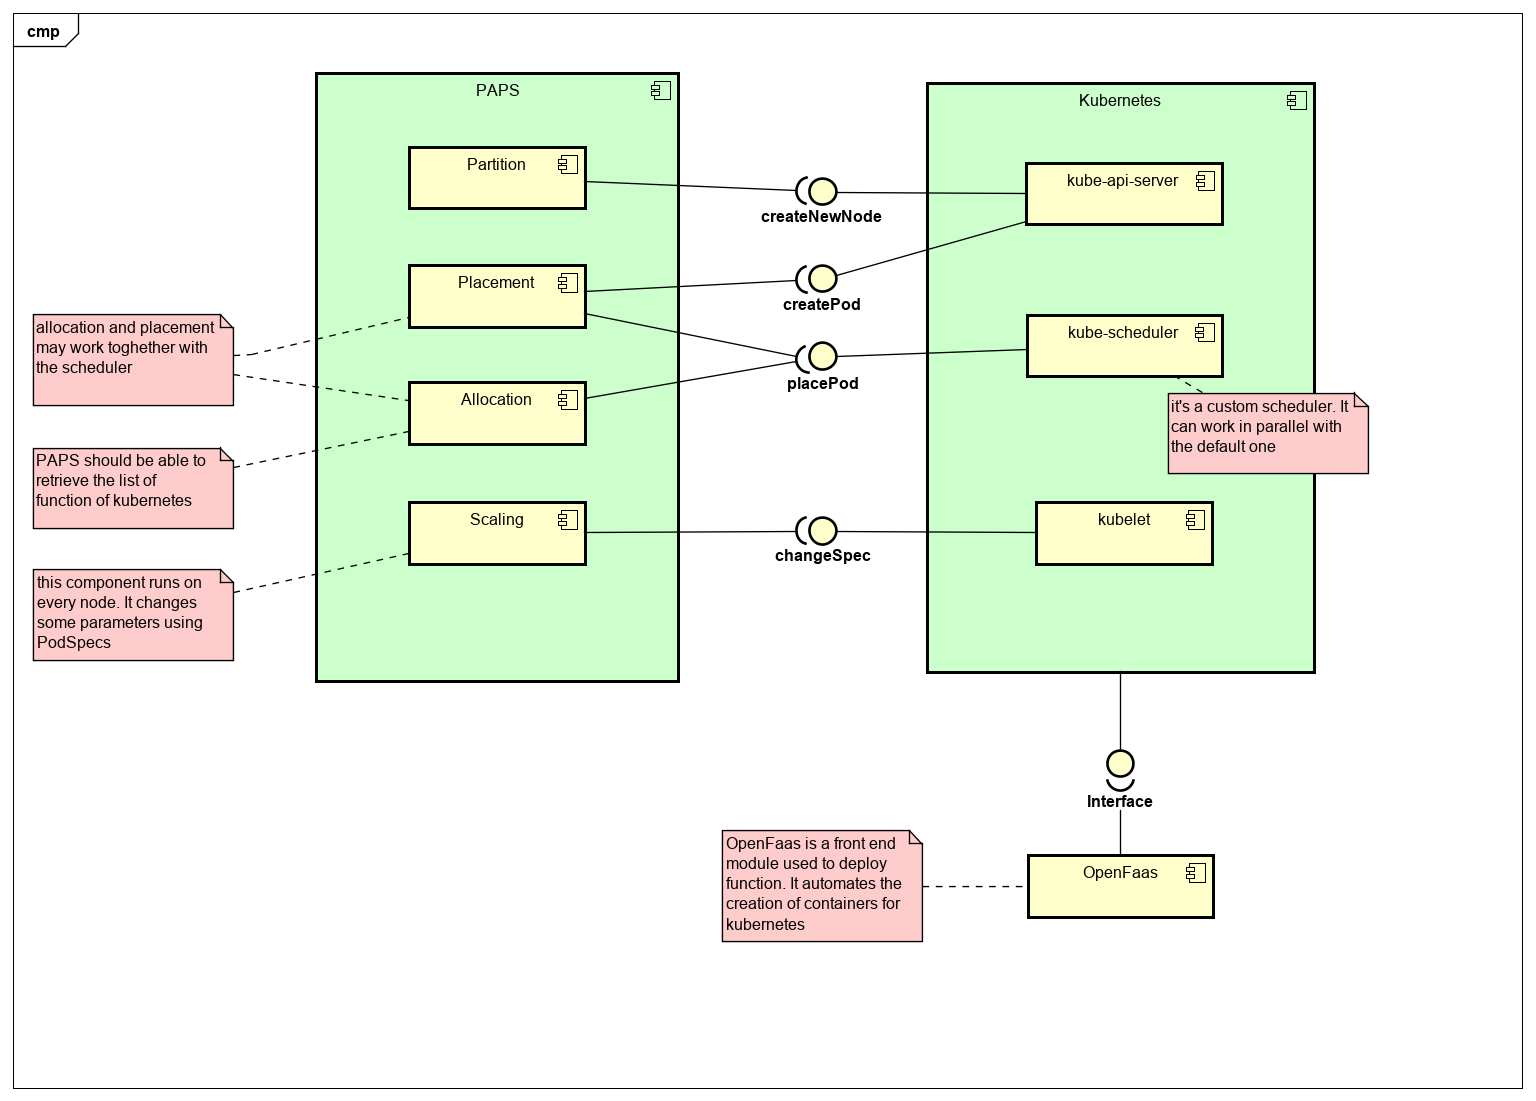
\includegraphics[width=\textwidth]{componentPAPS.png}
    \label{fig:component}
    \caption{Component diagram of PAPS}
\end{figure}

The first of the four PAPS phases is the \textbf{partition}, in this phase the original 
network topology on which PAPS will need to work is divided into delay-aware communities in 
order to reduce the scope of the following parts. To do that the idea is to take as input a 
delay matrix describing the measured delay between the nodes of the networks and other 
additional parameters that can be useful to describe the desired behavior of the partitioner.
This input can be provided as a file input or even through the OpenFaas GUI and will than be
parsed by the program to fill some data structures. The partition will first of connect to 
kubernetes API manager and do a call to obtain the list of registered nodes to check if they 
match with what has been parsed from the input. This operation needs to be done in order to
avoid the presence of nodes in the topology that are not actually managed by kubernetes and 
so that can't be modified and labeled according to the specific needs. 

To divide the network the partition will use SLPA, an algorithm which uses label spreading 
techniques to decide to which community each node will belong. The main component of this 
algorithm is the memory inside each node, there it will store all the labels received and 
it will process them in each round to decide the label to spread and at the end of the 
process the final label which will identify the community. Since the initial idea of this 
algorithm was developed to divide social networks profiles in communities, it can create 
overlapping node which will belong to more than one community. For our implementation this
is a problem but can be easily solved in many ways. Since all the labels kept at the end 
of the process are valid ones the simplest idea is to just randomly choose one of them or,
with some more processing, is also possible to pick the most popular one among all the 
remaining labels. In our implementation we select the first one in the list, which is 
equal to picking a random one since all the nodes are shuffled at each round, but it can 
be easily changed by changing few lines in the SLPA code.

\begin{figure}[h]
    \centering
    \subfloat[SLPA Pseudocode]{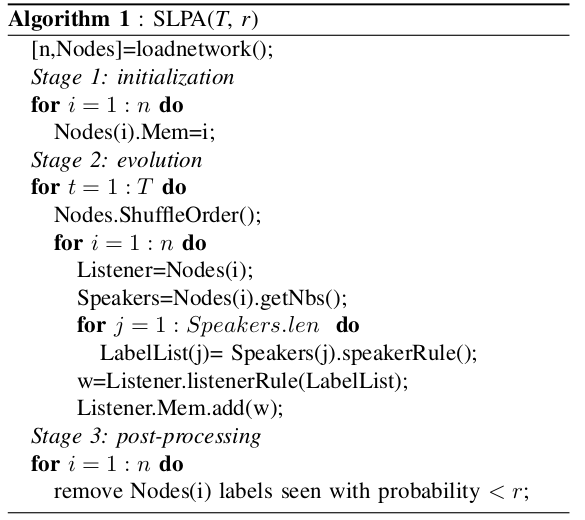
\includegraphics[width=.4\linewidth]{SLPAPseudocode.png}}%
    \label{fig:pseudocode}
    \subfloat[An example of communities division]{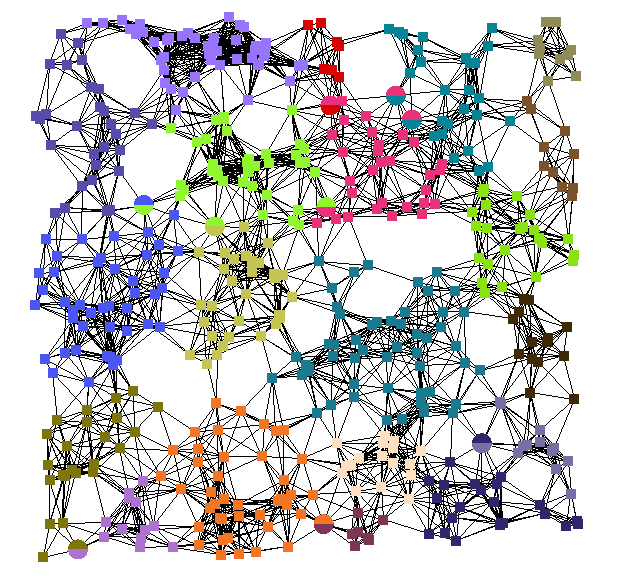
\includegraphics[width=.4\linewidth]{PPAP_communities.png}}
    \label{fig:communities}
\end{figure}

As an additional division tool the Partition keep the size of the communities under control
applying Round Robin to oversized communities to split them in smaller ones and have all 
communities under a given threshold size.\\

Once the network is split in communities, in each one the \textbf{allocation} phase will take
place. There the community leader will compute the resource allocation to assign to each node
according to the current load of the network and to respect the SLA of each function deployed.
To do that a MIP model is solved internally, using the IBM solver \footnote{IBM ILOG CPLEX 
Optimization Solver: https://www.ibm.com/products/ilog-cplex-optimization-studio}, stored in 
a dedicated container inside the leader node. Since it is inside the community leader, it 
will need to have access to some performance metrics regarding the other nodes of its community
and this can be easily done through the kubernetes API by filtering with the correct community
label. The result of the allocation will tell how many pods of each function will be scheduled
on each node in order to meet the SLA for all the received request at that moment.
The allocation phase will be periodically triggered to check if the provided allocation
schema is still valid or needs to be changed. \\
All the nodes will also implement an internal allocation phase which will change the amount 
of resources assigned to each scheduled pod inside the node itself since between two 
allocation cycles the amount of resources needed to meet the SLA of each function will 
slightly change. To do that a pod for the allocation will be always deployed in each node
and it will contain a function which works only on local resources.\\

The allocation phase will work in combination with the \textbf{placement} phase using a
\textit{kube-scheduler} module to actually deploy the pods necessary to meet realize the 
computed model. The kube-scheduled will be a custom module running in the network and will
contain some rules on how to deploy pods according to the MIP result. To correctly schedule 
pods, the filtering rules of the scheduler will be modified to filter by community and for 
a particular node in the community. Once the correct node is identified, the scheduler will 
actually deploy the pod in the node and from now on it will be up and running and ready to 
be used. \\

The last phase is the \textbf{scaling} which will use a PID controller to keep meeting the
SLA of all the functions on each node. Since this is a node level function, it will be
deployed in a pod on each node, maybe together with the allocation part, and will be always
up to check the resource utilization. This part will trigger the kubelet module of kubernetes
by changing the PodSpec relative to the deployed function if needed to keep the performance
under the given SLA. If a more drastic change is identified, it will make a call to the 
leader and ask for a new MIP evaluation even before the normal control period. 


